% #############################################################################
% This is Chapter 1
% !TEX root = ../main.tex
% #############################################################################
% Change the Name of the Chapter i the following line
\fancychapter{Introduction}
\label{chap:intro}
\cleardoublepage
The way we have been using and producing energy so far has been contributing to climate change and global warming. In 2016, the largest contributor to the Portuguese emissions was indeed the Energy sector (accounting for almost 70\% of total emissions)\cite{NacionalReport} .


Reducing consumption, increasing the share of renewables in the energy mix, and improving efficiency \cite{Europa1, Europa2, Europa3}, are among the main measures established by the \ac{EU} in order to achieve its long-term goal of reducing greenhouse gas emission and thus turning Europe into a low-carbon economy \cite{Europa2050}.


Several solutions proposed in the areas of \ac{HCI} and \ac{ICT} can be adapted to help reach the above--mentioned sustainability goals. Power Share, which is the work described here, leverages on some of them - namely \ac{EFT} and \ac{ET} via blockchain (a review on \ac{EFT} and \acp{ETS} is provided in \cref{chap:back}) - and was implemented as part of \ac{SMILE}, an EU H2020 funded research project.



 %\enquote{Cras gravida, diam sit amet rhoncus ornare, erat elit consectetuer erat, id egestas pede nibh eget odio.}
%\acp{WLAN} plural

% #############################################################################
\section{Eco Feedback Technology}

Reducing energy consumption is a critical step in lowering greenhouse gas emissions. Nevertheless, many people are not yet open to change their energy consumption patterns. This is mainly due to the fact that, despite energy monitoring and billing, households are largely unaware of the magnitude and impact of their own consumption. Energy is indeed perceived differently to other resources: it is invisible and its abstract nature leads people to underestimate the amounts of energy involved in their daily domestic practices \cite{ReducingDomesticEnergy}.


\ac{ICT} research developed several technologies for supporting behavioral change towards sustainability, and \ac{EFT} - i.e. a technology that "provides feedback on individual or group behaviors with a goal of reducing environmental impact" \cite{Froehlich2010} - is one of them. \ac{EFT} aims to make consumption visible in terms of scale and impact, and its effectiveness (savings ranging from 5\% to 15\%) has been demonstrated by over 40 years of research in multiple fields, from environmental psychology to \ac{HCI} \cite{Wang1990, Darby2006, Froehlich2010}.

% #############################################################################
\section{Energy Trading and the blockchain}

Due to decreasing prices of solar \ac{PV} equipment, the number of prosumers - “considered as regular households that consume and produce their own energy” \cite{Prosumers} - is growing exponentially. In Portugal, for instance, in 2015 the number of residential prosumers was 62.000, and it is expected to reach quota 88.000 by 2020 \cite{EuropeanComissionStudy}. Till now, prosumers had a limited control over their surplus energy. They could buy a \ac{BESS} to store the surplus energy and use it later (for example, during peak hours when the energy cost is higher) or sell it back to the electricity supplier against payment of a fixed fee.



Nowadays, thanks to the development of blockchain technology (better described in \cref{chap:back}), prosumers can finally sell their surplus energy to neighbors who are in an energy deficit. Blockchain consists in "an open, distributed ledger that can record transactions between two parties efficiently and in a verifiable and permanent way. The ledger itself can also be programmed to trigger transactions automatically" \cite{TruthBlockchain}, through the so--called smart contracts. Despite \ac{P2P} technologies, \ac{ET} was already possible without blockchain. Such technologies could provide great benefits to the energy industry and has the potential to disrupt the market. Blockchain technology is indeed "the only solution for a full \ac{P2P} market" \cite{Powerledger} and is especially needed when there are multiple parties transacting in near real-time, as it is the case of the energy sector. Through blockchain, third-party intermediaries are no longer required, which, in turn, leads to a decrease in transactions costs and time thus allowing small subjects, like prosumers, to enter the energy market.
\ac{P2P} \ac{ET} does not only represent an opportunity for prosumers but also for consumers,\acp{DSO} and \acp{TSO}. Indeed, blockchain technology enables dynamic pricing, flexibility, and adds transparency (since data about transactions are stored in a decentralized fashion ensuring data security and greater independence from a central authority). This way, customers have more control over the price they sell their surplus energy for and can benefit from instant billing settlement. Ultimately, smart contracts on the blockchain can be used to balance demand and supply. Therefore, such a system has the potential to increase grid balance \cite{PeerToPerrEnergyTrading} and share of renewables in the energy mix, while radically changing the energy market.



The number of projects and blockchain startups in the Energy area increased significantly in the last years, demonstrating that \ac{P2P} \ac{ET} via blockchain can be a viable solution for the development of an actual microgrid - “a local energy grid with control capability, which can disconnect from the traditional grid and operate autonomously” \cite{HowMicrogridWorks}.


\section{Demand Response and Energy Storage Systems: the SMILE project}

The SMILE project aims to demonstrate a set of both technological and non-technological solutions targeting the distribution grid to enable demand response, smart grid functionalities, storage, and energy system integration.



The consortium is composed by 19 partners from 6 EU countries, all working on three large-scale pilot projects that will be implemented in three different European islands - Madeira, Orkney and Samsø - which have similar topographic characteristics but different policies, regulations, and energy markets. Each demonstrator will test a different combination of technological solutions according to local specificities and the existing infrastructure, involving all value chain actors needed to efficiently implement these solutions. The overall objective is to pave the way for their introduction in the market in the near future, while establishing mutual learning processes and providing best practice guidance for replication in other regions. The Madeira demonstrator consists of three different pilots, aimed respectively at:

\begin{enumerate}
\item Optimizing self-consumption of solar energy;
\item Providing frequency and voltage control mechanisms;
\item Implementing a low-cost smart charging solution for \acp{EV}.
\end{enumerate}

Power Share was designed as a possible future business model for one of the solutions deployed for the purpose of the SMILE project, specifically, the one targeting the optimization of self-consumption (described below). For more information about the other SMILE pilots, please, visit \url{http://www.h2020smile.eu}.


\subsection{Pilot one: Optimizing self-consumption}

As stated above, the three pilots will test the most appropriate solutions according to local specificities and conditions. On this respect, the case of Madeira represents a critical energy challenge as it is a truly independent system with a small--scale and wholly isolated electric grid. That is to say, Madeira is a perfect energy island, in which all the energy is generated locally.



Currently, there is already an average of 30\% of renewables in the grid but one of the main objectives of the local \ac{DSO} is increasing the injection of renewables. As such sources can amount to an increase in provisioning security and efficiency benefits. At the same time, the instability of these sources represents the main blocking force for their penetration, especially in the case of a small scale and completely isolated grids like the one of Madeira.


The typical southern Mediterranean climate with high solar radiation characterizing Madeira, makes the Island a promising location for \ac{PV} usage. However, the increase of solar energy represents a challenging business case for the local \ac{DSO}, as it tends to result in the phenomena of \ac{VI} and \ac{FF}. Also, the fuzziness of the generation of \acp{PV} makes even more difficult the matching between generation and load demand, which leads to interruptions and lousy power quality. The frequency stability issue puts the strain on the distribution grid and security of supply and leds to the need of avoiding direct injection to the grid. Thus, in order to protect the grid from the impact of variations in the solar \ac{PV} production, since 2014 new solar \ac{PV} installations are only allowed in self-consumption mode and without injection to the grid. This imposition helps to maintain a stable grid but is preventing the local \ac{DSO} from achieving the desired 50\% share of renewables in the mix by 2020.


\begin{figure}[h]
\centering
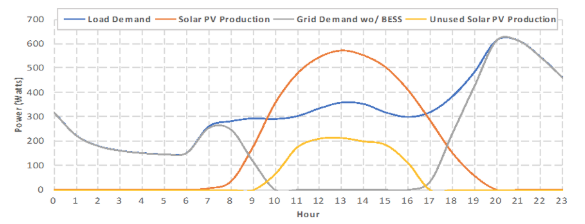
\includegraphics[width=1\textwidth]{./Images/grafico_intro}
\caption{Average household production and consumption in Madeira}
\label{fig:graph_intro}
\end{figure}

As it can be observed in \Cref{fig:graph_intro}, for the average household in Madeira, the production of solar energy is higher when the consumption is lower. Indeed, the peak consumption usually happens between 7 PM and 9 PM, which is the periods of highest domestic demand. Consequently, in self-consumption only scenarios, there is usually a considerable waste of renewable energy. 


This is the issue that will be addressed by the first pilot of \ac{SMILE}, which is targeted at both domestic and commercial \acp{UPAC}. The goal here is to equip these installations with BESS and specialized \acp{BMS} to maximize the self--consumption of those installations.


\section{Power Share}
The Power Share project was designed to test a future business model for the pilot of \ac{SMILE} described previously. Therefore, it assumes a scenario where several solar prosumers are equipped with a \ac{BESS}.
The main goal of this project is developing an end-user application for \ac{ET} that uses blockchain as a payment method and contemporarily provides \ac{EF} through a low-cost and easy to use the system. It is designed to be inclusive, that is to say, it does not target only prosumers but also consumers. By combining \ac{ET} with \ac{EF} we aim to:

\begin{itemize}
\item Foster learning and raise awareness about people energy use;
\item Allow prosumers to further benefit from their surplus energy and foster them to engage in \ac{ET} toward the common good;
\item Increase the share of RES in the energy mix by allowing consumers in need of energy to buy local, green energy from their neighbors. Through Power Share they can have control over price and source of their power.
\end{itemize}


The application was field-tested in 9 households in Funchal (Madeira), with the support of the research team from the \ac{M--ITI} working on SMILE, whose members helped with participants recruitment and the installation of smart meters and communication infrastructure in each household.
In this respect, it should be pointed out that all transactions carried out through the app will be simulated by the server. This is due to the fact that all prosumers participating in the field-test installed their \ac{PV} power system after 2014, therefore are not allowed to inject the surplus energy to the grid.



Such limitation represents the big potential of a system like Power Share. Indeed, if results from the field-test show that the local community is prone to adopt \ac{ETS}, it could become a viable solution for the local \ac{DSO} to manage and distribute an increased amount of \acp{DER}, while contributing to maintain grid stability. For example, by leveraging blockchain smart contracts, Power Share could enable prosumers to sell stored energy when the market most needs it, thus helping to reduce strain across the grid and make it more efficient for all.
It our opinion testing this virtual, local microgrid represents a first step towards the development of a smart distributed grid -  “an electricity network that can intelligently integrate the actions of all users connected to it - generators, consumers and those that do both - in order to efficiently deliver sustainable, economic and secure electricity supplies” \cite{OverviewSmartGrid} - in Madeira Island.


In this respect, the field-test of Power Share has a twofold goal:

\begin{itemize}
    \item On the one hand, it is meant to assess users acceptance of \ac{ET} in a smart-grid scenario in order to understand if it could be a viable future business model  for one of the solutions developed in the scope of the SMILE project;
\item On the other hand, it aims to evaluate users understanding  and attitudes toward adoption of blockchain as a payment method.
\end{itemize}


At the time of this writing, the application field-test is ongoing. Since it will end after the deadline for the submission of this document, results from the semi-structured interviews about users acceptance of the system won’t be included in this report. Nevertheless, users interactions with the app are being monitored through Fabric, a platform for developers made for that purpose. Preliminary results from the analysis of three-weeks data are provided in \cref{chap:evaluation}.

The present document is structured as follow: \Cref{chap:back} provides a review of the work done so far on both \ac{EFS} and \ac{ET} areas, analyzing research and commercial projects. \Cref{chap:implement} presents the architecture of the solution proposed here, describing the rationale behind it, as well as front- and back-end design and implementation stages.
\cref{chap:evaluation} focuses on project evaluation providing some preliminary results. \Cref{chap:conclusions} presents results, limitations and future work.


